\documentclass[11pt,a4paper]{article}
\usepackage[utf8]{inputenc}
\usepackage{amsmath}
\usepackage{amsfonts}
\usepackage{amssymb}
\usepackage{enumitem}
\usepackage{listings}
\usepackage{xcolor}
\usepackage{graphicx}
\usepackage{url}
\usepackage{subfigure}
\usepackage{xspace}
\lstdefinelanguage{MySketch}%
{ mathescape,
  numbers=left,
  keywords={assume, assert, Array, Int, func, while,
  do, if, then, else, input, output, public, private, product, together, is,
  guard, instrument}
}

\definecolor{mGreen}{rgb}{0,0.6,0}
\definecolor{mGray}{rgb}{0.5,0.5,0.5}
\definecolor{mPurple}{rgb}{0.58,0,0.82}
\definecolor{backgroundColour}{rgb}{0.95,0.95,0.92}


\lstset{
    % backgroundcolor=\color{backgroundColour},
    commentstyle=\color{mGreen},
    keywordstyle=\color{magenta},
    numberstyle=\tiny\color{mGray},
    stringstyle=\color{mPurple},
    basicstyle=\footnotesize\fontencoding{T1}\ttfamily,
    breakatwhitespace=false,
    breaklines=true,
    captionpos=b,
    keepspaces=true,
    numbers=left,
    numbersep=5pt,
    showspaces=false,
    showstringspaces=false,
    showtabs=false,
    tabsize=2,
    language=C
}

%%
%% Referencing in a space-saving manner
%%
\newcommand{\secref}[1]{\S\ref{sec:#1}}
\newcommand{\appref}[1]{Appendix~\ref{sec:#1}}
\newcommand{\subsecref}[1]{\S\ref{subsec:#1}}
\newcommand{\figref}[1]{Fig.~\ref{fig:#1}}
\newcommand{\algref}[1]{Alg.~\ref{alg:#1}}
\newcommand{\tabref}[1]{Table~\ref{tab:#1}}
\newcommand{\codetext}[1]{\texttt{#1}}
\newcommand{\ctVerif}{\texttt{ct-verif}\xspace}
\makeatletter
\newcommand\module{\@startsection{paragraph}{4}{\z@}%
                                    {1.25ex \@plus1ex \@minus.2ex}%
                                    {-1em}%
                                    {\normalfont\normalsize\slshape\bfseries}}
\makeatother

\title{Review: Verifying Constant-Time Implementations}
%\subtitle{Formal Verification Background Paper Report}
\author{Mahyar Emami, Rishabh Iyer, Sahand Kashani \\ firstname.lastname@epfl.ch}

\begin{document}
\maketitle

\section{Introduction}
% Say a few general words about the general context of the paper you chose. Explain why the topic is of interest, or where it can be applied. If it is about a piece of software or artifact, give a description of it. State the main result of the paper and why it is new or how it improves on previous state of knowledge. You can cite references using, for example \cite{BibliographyManagementLaTeX} and make a succint presentation of the organisation of your report.

Timing attacks---attacks that extract secrets by measuring timing differences under adversary-controlled inputs---on cryptographic libraries~\cite{bernstein_cache_timing_attacks, dsa_exponentiations} pose a major challenge to information security today. 
Popular cryptographic libraries (e.g., OpenSSL~\cite{openssl}) run on millions of devices; hence a vulnerability in such a library has the potential to compromise all such devices simultaneously.

Constant-Time programming is the most effective software countermeasure against such attacks.
Constant-time programming involves rewriting a program such that (1)~its control flow does not depend on program secrets, (2)~it does not perform any secret-dependent memory accesses, and (3)~it does not use variable-latency instructions to operate on secrets.

However, it is challenging to write and/or reason about constant-time programs are hard since it typically involves the use of low-level programming languages and programming practices that deviate from software engineering principles.
For example, two constant-time violations\footnote{See pull requests \#147 and \#179 in ~\cite{s2n}} were found in Amazon's s2n library~\cite{s2n}soon after its release with the second exploiting a timing-related vulnerability introduced when fixing the first.

In this work, Almeida et. al~\cite{almeida} propose using formal methods to \emph{automatically} verify whether a program runs in constant time. 
To do so, they provide a precise framework to model constant-time properties(~\secref{prelimnaries}), a sound and complete reduction of constant-timeliness of input programs to assertion safety of a self-product(~\secref{body}) and design, evaluate an automated tool that verifies the constant-timeliness of cryptographic algorithms from widely used libraries within seconds(~\secref{eval}). 


\section{Preliminaries}

% State the technical details that are necessary to understand the paper. It is generally a collection of definitions, concepts and notations with potentially a few preliminary results. It can be, for example the mathematical framework in which the topic of your paper is expressed. In particular, fix the notation you will be using for your review.

\begin{itemize}
  \item Simple example that can easily be checked + example of benign branch that other tools cannot determine to be constant-time.
  \item Formalism used to model a program (while-language framework and what it supports).
  \item The paper proposes modeling contant-time verification of a program by encoding the input program as a safety condition and executing the program to check if it is safe.
  \item Define what leakage $L(c)$ is formally. A leakage model can either depend on
        \item \begin{enumerate}
          \item Path-based characterizaion of constant-time: leakage of branch conditions.
          \item Cache-based characterization of constant-time: leakage of memory access indices.
          \item Instruction-based characterization of constant-time: leakage of instruction operand sizes.
        \end{enumerate}
  \item Define what it means for a program to be safe (i.e., it does not violate an assertion inserted when the safety program).
\end{itemize}


\section{Redcuing security to safety}

% Explain the paper, in your own words. Don't go into as many details as the
% original text, but the person reading your review should have a general
% understanding of the paper's results and how those results can be obtained.
% The structure and content of this section of course heavily depends on the
% paper itself. Don't hesitate to split it in multiple sections or subsections,
% for example: \subsection{An algorithm for whatever problem we try to solve} If
% your paper contains theorems, sketch the proofs of important theorems.

% \subsection{Benchmarks} If it contains benchmarks, show the key scores or
% results.

% You can follow the structure of the paper you're reviewing, but write with
% your own words.

% \subsection{Reducing security to safety}

At the interface of any security-sensitive function call, there usually exists a
\emph{contract} that describes which inputs or outpus are deemed public (i.e.,
known to attackers) and which ones are private (i.e., to protect). A leak should
never reveal anyting about the private inputs and outputs (but publics ones 
can be leaked).
% If we denote a program as $p$ (with the usual definition of a prgram being a
% sequence of statements or programs) with a corresponding state $s$ (which
% is mapping from variables to values) then at each step of execution, from
% state $s$ executing program/statement $p$ we can define leakage $L(.)$ as follows:

% \begin{equation}
%     \begin{split}
%     L(\langle s, \text{\texttt{if}}~e~\text{\texttt{then}}~p_1~\text{\texttt{else}}~p_2 \rangle) = & s(e) \\
%     L(\langle s, \text{\texttt{while}}~e~\text{\texttt{do}}~p \rangle) = & s(e) \\
%     L(\langle s, x_0[e_0] = e \rangle) = & s(e_0)s(e_1)...s(e_n)
%     \end{split}
% \end{equation}

% The first two leakage sources correspond to leakage from control flow while the
% latter is leakage from memory access. Note that in the third leakage source,
% a memory leak $s(e_0)$ corresponds to leakage from the right-hand-side indexer
% expression and $s(e_1)$ to $s(e_n)$ possible indexer expression in expression
% $e$. We can also extend the leakage sources to comprise machine operations that
% have operand-dependent execution latency (i.e., division in x86).

Using the leakage rules in \secref{prelimnaries}, 
we can reduce constant-time security to execution safety (i.e., termination
without any failed assertions) by building a \emph{self-product} in which two
abstract execution take place back to back, only differing in the value of
private inputs and outputs. \figref{rules} shows how a program product can
be constructed where $\hat{p}$ is the program $p$ with all variables renamed
(i.e., an alternative execution).

\begin{figure}[h]
    \centering
    \subfigure[Program product construction rules]{
        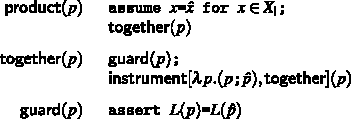
\includegraphics[width=0.45\textwidth]{./figs/fig_7.pdf}
    }\label{fig:fig_7}
    \subfigure[Instrumentation rules] {
        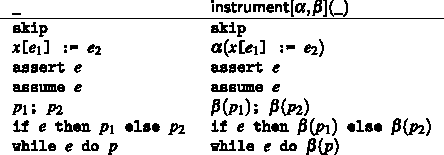
\includegraphics[width=0.45\textwidth]{./figs/fig_8.pdf}
    }\label{fig:fig_8}
    \caption{Program product}
    \label{fig:rules}
\end{figure}

\begin{figure}[t]
    \lstinputlisting[language=C]{example.c}
    \caption{Running example - sub-array copy}
    \label{fig:example}
  \end{figure}

The essence of the transformation is the instrumentation, which reduces 
constant-time security to assertion safety. \figref{example_prod} shows 
the product of the sub-array copy program in \figref{example}. Notice how
the program is instrumented with assertions to ensure leakage remains the same at
every step of execution. In this example, the private inputs \texttt{l\_idx} and
its renaming are not assumed to be equal, therefore the assetion on line 8 fails
and the program is proved to be unsafe and hence it follows that the program is
not constant-time secure.

\begin{figure}[h]
    \lstinputlisting[language=MySketch]{prod.my}
    \caption{example program product of the sub-array copy program.}
    \label{fig:example_prod}
\end{figure}



\section{Discussion}\label{sec:discussion}

\texttt{ct-verif} operates at the level of LLVM bitcode and can therefore only formally attest to whether a program's
representation as bitcode is constant-time.

Translating a bitcode program into binary is a straightforward process and is generally a simple one-to-one mapping between bitcode instructions and assembly.
In theory an assembly program should therefore preserve the constant-time property if the source LLVM bitcode is proven to be constant-time.

However, while this argument does hold for simple RISC-like ISAs, it does not for complex CISC-like machines like the x86 architecture.
There is in reality no true ``x86'' machine as no x86 processor actually executes the CISC instructions it receives as input directly.
Instead, these CISC instructions are decomposed into RISC-like $\mu$Ops before being scheduled for execution on a RISC-like backend.
This decomposition is handled transparently by microcode sequencers in the CPU's frontend and is not under the control of the user as microcode updates can change instruction behavior.
Asserting that a constant-time LLVM bitcode program remains constant-time when translated to x86 assembly is unclear as users have no way of knowing how an instruction is decoded into $\mu$Ops.

The \texttt{dudect} project appeared after \texttt{ct-verif} and suggested the only way to decide whether a program is constant-time or not is to actually run it and time its execution~\cite{dudect}.
The main idea behind \texttt{dudect} is to run a supposedly constant-time program under two environments and measure its execution time: (1) using \textcolor{red}{fixed} secret inputs, and (2) using \textcolor{blue}{random} secret inputs.
If the program is constant-time, then the timing traces of these two programs should be indistinguishable.
However, machines do not have deterministic execution times due to caches and OS scheduling, so relying on the execution time alone to determine constant-timeness would be incorrect.
\texttt{dudect} therefore proposes using a statistical method---an ``equivalence of means'' $t$-test---to determine whether multiple program executions under the two aforementioned environments are statistically indistinguishable.
If yes, then the program is \emph{possibly} constant-time. If not, then the program is \emph{definitely not} constant-time.
Combined with a formal constant-time proof obtained from \texttt{ct-verif}, the mechanism proposed by \texttt{dudect} can validate that the $\mu$Op decomposition of a program is constant-time.

We evaluated the \texttt{dudect} method on 9 examples from the \texttt{ct-verif} paper and were able to validate their constant-time property.
In fact, \texttt{dudect}'s method of operation lends itself well to a graphical validation when a constant-time violation is detected.
Indeed, repetitively running the program with fixed/random private inputs and plotting the CDF of its average execution time generates curves that should perfectly overlap if the program is constant-time\footnote{We modified \texttt{dudect} to automatically extract and plot its timing information.}.
Figure~\ref{fig:dudect_donna} shows an example of running the \texttt{dudect} method on two implementations of \texttt{curve25519} that differ in the constant-time property.

\begin{figure}[h!]
  \centering
  \subfigure[Non-CT implementation]{
      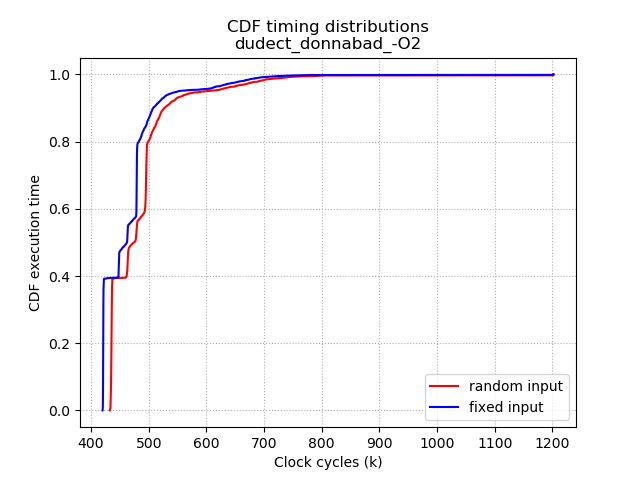
\includegraphics[width=0.45\textwidth]{./figs/donnabad_cdf.png}
  }\label{fig:dudect_donnabad}
  \subfigure[CT implementation] {
      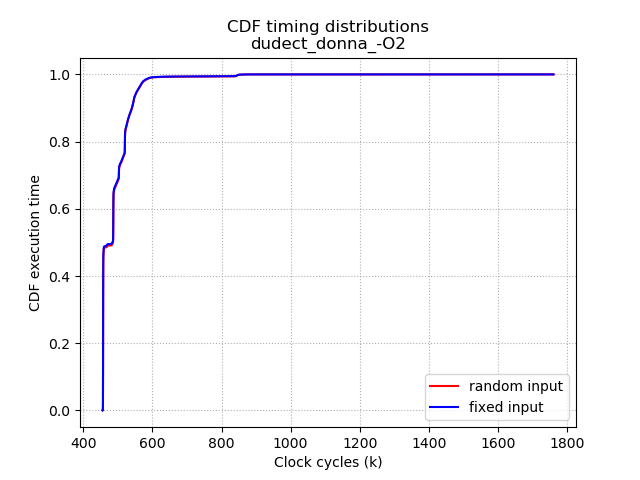
\includegraphics[width=0.45\textwidth]{./figs/donnagood_cdf.png}
  }\label{fig:dudect_donnagood}
  \caption{CDF timing behavior of a non-CT vs CT implementation of an elliptic curve.}
  \label{fig:dudect_donna}
\end{figure}

Figure~\ref{fig:dudect_sha} in turn shows how an example that a formal tool could not prove as constant-time \emph{could} be constant-time since the execution curves overlap perfectly.

\begin{figure}[h!]
  \centering
  \subfigure[SHA256]{
      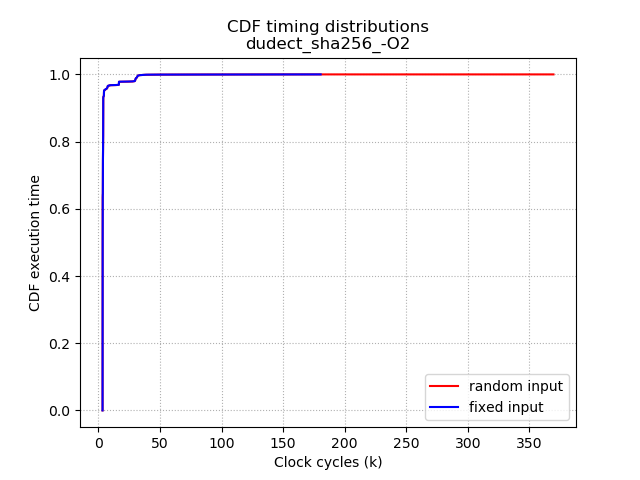
\includegraphics[width=0.45\textwidth]{./figs/sha256_cdf.png}
  }\label{fig:dudect_sha256}
  \subfigure[SHA512] {
      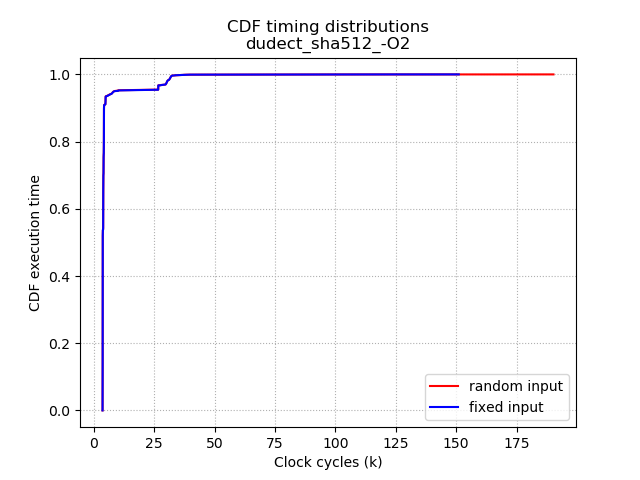
\includegraphics[width=0.45\textwidth]{./figs/sha512_cdf.png}
  }\label{fig:dudect_sha512}
  \caption{CDF timing behavior of \texttt{libsodium}'s SHA256/SHA512 implemenation. Both are statistically constant-time.}
  \label{fig:dudect_sha}
\end{figure}

% The \texttt{ct-verif} tool was released in 2016, two years before widespread micro-architectural side-channel attacks like Meltdown~\cite{meltdown} and Spectre~\cite{spectre} were reported.
% Formal techniques are, in theory, able to detect whether a program is vulnerable to certain categories of side-channel attacks.
% A program's constant-timeness property can be formally verified, but only if one assumes the program model is correct.
% Indeed \texttt{ct-verif} uses LLVM's operation cost model to determine whether an instruction
% The disclosure of such attacks encourages the use of formal techniques to verify a design's implementation

\section{Tool Implementation}

\ctVerif is an open-source implementation of the constant-time verifier we
described earlier in \secref{body}. \figref{ct-verif-flow} illustrates the
tool flow from top to bottom. To prove constant-time security, a C function is
instantiated in a proof harness that categorizes inputs and outputs as public/secret. Then,
the function and its harness are compiled down to \codetext{llvm} bitcode. The
bitcodes are linked together and converted to \emph{Boogie Programming
Language} (\codetext{.bpl}). Compilation down to \codetext{.bpl} is automated
through \emph{SMACK}~\cite{smack}, but it is possible to customize the flow if
needed and only rely on the the \codetext{bitcode}-to-\codetext{bpl} conversion
of SMACK.

The linked \codetext{bpl} files are then fed to \emph{BAM! BAM! Boogieman} which
performs the key task of generating the self-product (c.f. \secref{body}), and
finally the self-product---which contains assertions and assumptions---is
given to \emph{Boogie}~\cite{boogie} to verify assertion safety.


\begin{figure}[h]
    \centering
    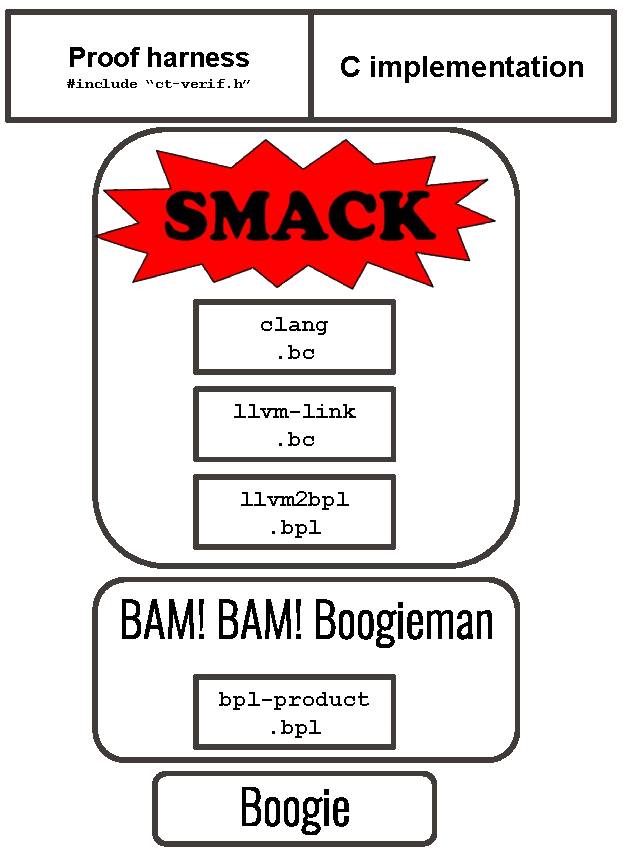
\includegraphics[height=0.4\textheight]{figs/ct-verif-flow.pdf}
    \caption{\ctVerif tool flow}
    \label{fig:ct-verif-flow}
\end{figure}




To ensure the tool works as advertised, we first tried proving/disproving
small examples with obvious answers before reproducing the
results reported in the paper~\cite{almeida}.


\subsection{Handling toy programs}

We started by disproving constant-timeness of the code given in \figref{example}.
\ctVerif correctly identifies this code as unsafe (i.e., not constant-time).
The test harness for this examples is a simple wrapper that declares all inputs
as public except \codetext{l\_idx}.

\begin{figure}[h]
    \centering\resizebox{0.7\columnwidth}{!}{\lstinputlisting[language=C]{code/example_wrapper.c}}
    \caption{Proof harness for sub-array copy in \figref{example}.}
    \label{fig:example_wrapper}
\end{figure}

A more interesting example is the slightly unusual \codetext{vector\_add}
function in \figref{vector_add}. Notice how by declaring \codetext{a[N - 1]} as
a public input we make the code constant time. \ctVerif also successfully
identifies this code as constant time. Now if we remove the public input
declaration on line 10, then the code will no longer be constant time because the
for loop will leak the length of arrays and \ctVerif also correctly marks the
program as non-constant time.

\begin{figure}[h]
    \centering\resizebox{0.7\columnwidth}{!}{\lstinputlisting[language=C]{code/vector_add.c}}
    \caption{A slightly unusual vector addition.}
    \label{fig:vector_add}
\end{figure}


\subsection{Reproducing results}


We set out to reproduce all the results in the paper, however, we ended up
only verifying some of them. There were two reasons:
\begin{enumerate}
    \item Functions reported as constant-time in the paper could not be proven
    to be constant-time using \ctVerif;
    \item The reported functions could not be found in the \ctVerif repository,
    or their build procedures were broken/incomplete.
\end{enumerate}

\subsubsection{\codetext{tea}}
\codetext{tea} is a tiny encryption algorithm that consists of about 20 lines
of code. We successfully verified \codetext{tea} to be constant-time.



\subsection{\codetext{libfixedpointfixedtime}} \codetext{libfixedpointfixedtime}
is a library that implements a large variety of fixed-point arithmetic
operations in constant-time. The paper only reports constant-timeness for 10
functions in the library, but we managed to verify an additional 24 functions using \ctVerif
that were not reported in the paper. These additional functions are:
\codetext{fix\_is\_neg},
\codetext{fix\_is\_nan},
\codetext{fix\_is\_inf\_pos},
\codetext{fix\_is\_inf\_neg},
\codetext{fix\_eq},
\codetext{fix\_eq\_nan},
\codetext{fix\_ne},
\codetext{fix\_cmp},
\codetext{fix\_le},
\codetext{fix\_ge},
\codetext{fix\_lt},
\codetext{fix\_gt},
\codetext{fix\_neg},
\codetext{fix\_abs},
\codetext{fix\_add},
\codetext{fix\_sub},
\codetext{fix\_mul},
\codetext{fix\_div},
\codetext{fix\_floor},
\codetext{fix\_ceil},
\codetext{fix\_ln},
\codetext{fix\_log2},
\codetext{fix\_log10},
\codetext{fix\_convert\_from\_int64},
\codetext{fix\_convert\_to\_int64},
\codetext{fix\_round\_up\_int64},
\codetext{fix\_ceil64},
\codetext{fix\_floor64},
\codetext{fix\_sin},
\codetext{fix\_cos},
\codetext{fix\_tan},
\codetext{fix\_exp},
\codetext{fix\_sqrt},
\codetext{fix\_pow}.

\subsubsection{\codetext{curve25519-donna}} We successfully re-verified the C
implementation of the \codetext{curve25519-donna} elliptic curve. This function
was the hardest among all and took the longest time to prove (about 7 minutes).


\subsubsection{\codetext{libsodium}} \codetext{libsodium} is an easy-to-use
encryption library. We attempted to verify 4 functions here (\codetext{chacha20,
salsa20, sha256, sha512}). We used the Makefiles
provided by \ctVerif which isolate the C files used by each function (i.e., the
whole library is not compiled to \codetext{llvm} bitcode). We successfully
reproduced the paper results by verifying constant-timeness of
\codetext{chacha20} and \codetext{salsa20}, but failed prove it for
\codetext{sha256} and \codetext{sha512} (unlike what the paper claims).


Upon inspecting the C implementation of \codetext{sha256} and \codetext{sha512}
we couldn't identify exactly why these two functions are not constant-time.
This implored us look for other methods of asserting constant-timeness which
we will follows up on in \secref{discussion}.



\subsection{Scalability of \ctVerif}

To evaluate the scalability of this tool we first tried to verify
constant-timeness of function \codetext{s2n\_verify\_cbc} from Amazon's
\codetext{libs2n} library. The test harness for this function is included as one of the
examples in the \ctVerif repository but it had a simple bug where the test
harness was calling itself instead of the \codetext{s2n\_verify\_cbc} function.
However, there was no build script for this specific function and we had to modify the
\codetext{Makefile}s in the \codetext{libs2n} library to generate
\codetext{llvm} bitcode instead of a binary. We then manually linked the bitcode
library with the test harness and invoked \codetext{llvm2bpl} pass---provided by
SMACK---and fed the generated \codetext{.bpl} files to BAM! BAM! Boogie to
generate the program product. Unfortunately. \codetext{llvml2pl} resulted in
many warnings regarding memory safety and self-product program generation failed
to due an resolved reference.


In another attempt, we compiled the OpenSSL library down to \codetext{llvm}
bitcode to verify the SHA-1 function. Transformation from bitcode to bpl
resulted in over 70GiB of memory usage and did not terminate after 30 minutes.


Unlike the functions verified in the paper, these two functions are not
isolated and the bitcode given to \ctVerif contains unused code. It seems like
SMACK transforms the whole program irrespective of the target function. This
approach limits the usability of \ctVerif since verifications requires a good
understanding of the underlying library structure to be able to isolate the used
code.


% \section{Evaluation}
\label{results}

The authors implement the algorithm outlined in \secref{body} in a publicly available tool called \texttt{ct-verif}~\cite{ct-verif-github}. 
\texttt{ct-verif} takes as input the LLVM implementation of a cryptographic algorithm and outputs either a proof of constant-timedness or a counter-example showing how the property is violated. 
Under the covers, \texttt{ct-verif} leverages the SMACK verification tool~\cite{smack} to translate the LLVM to Boogie~\cite{boogie} code. 
It then performs its reduction on the Boogie code and applies the Boogie verifier to the resulting program. 

The authors evaluate their tool on examples from widely used cryptographic libraries including OpenSSL~\cite{openssl}, NaCl~\cite{nacl}, FourQlib~\cite{fourqlib} and \texttt{curve25519-donna}~\cite{donna}. The examples include encryption algorithms, hash functions, fixed-point arithmetic and elliptic-curve arithmetic. 
The size of the examples ranges from $50-1200$ lines of C code.

The authors demonstrate that \texttt{ct-verif} is typically able to verify that the examples are constant-time secure within seconds---most functions require $\leq 30s$ while the largest function requires $273s$. 
These results show that \texttt{ct-verif} can be easily integrated into the day-to-day development of cryptographic algorithms. 

% \section{Takeaways}

This work formalizes the previously imprecise notion of constant-time programming, in addition to providing a publicly available and fully automated tool can verify (in seconds) whether implementations of cryptographic algorithms from off-the-shelf libraries adhere to the notion of constant-time. 
This is, undoubtedly, an impressive result.

That said, the paper does have a few weaknesses: \\
\indent Firstly, \texttt{ct-verif} requires LLVM implementations which is problematic for two reasons.
Cryptographic code is often written directly in assembly due to the performance benefits. For instance, Vale~\cite{vale} demonstrates that OpenSSL assembly implementations outperform their C counterparts by up to 50\%.
Further, verifying that LLVM code runs in constant-time does not guarantee that the executable runs in constant time~\cite{KaufmannPVV16}. To the authors' credit, they do discuss such scenarios.

Secondly, the formalization of constant-time as presented by the papers is significantly weakened by the advent of micro-architectural attacks (~\cite{meltdown,spectre}). To be fair to the authors, such attacks became popular after their paper was published. Further, one could argue that such attacks are not a property of the implementation per-se, and are a menace that the underlying hardware/operating system must tackle.

Finally, the authors do not present a single example where their ``automated'' approach fails to verify constant-timedness in reasonable time. As such, the results look a little too good to be true. 

During the course of this project, we plan to investigate the first and third aspects of \texttt{ct-verif} more thoroughly. 
Specifically we aim to identify where the tool falls short and also patch it with LLVM-passes that can preserve constant-timedness. 

\bibliographystyle{plain}

\bibliography{biblio.bib}

\end{document}
